\clearpage
\begin{flushright}
    \textit{Лекция №21}
    \textit{2015.12.01}
\end{flushright}

\section{Монолитное ядро}

Переходим к подробному изучению монолитного ядра.
Примеры таких систем: Windows. Windows 2000 – не ялвяется ОС на основе микроядра в классическом понимании (стр. 25).
ОС Матч реализует крошечное ядро микроядра, но оно не эффективно. 
В Unix/Linux ядро - минимизировано.
Для ОС с монолитным ядром характерна система прерываний. 

Принято различать такие синхронные события:
\begin{enumerate}
    \item системные вызова (выполняются в процессе выполнения программы, которой требуется сервис системы; частыми являются обращение процессов к внешним устройствам (если речь идет об интерактивных процессах, то это клавиатура и мышь))
    \item исключения:
    \begin{enumerate}
    	\item  исправимые (страничные прерывания, которое возникает при отсутствии страницы в физической памяти, но в результате обработки этого исключения, вызывается менеджер памяти, который загрузит её в память)
    	\item  неисправимые, приводят к завершении программы с сообщением об ошибке.
	\end{enumerate} 
\end{enumerate} 

Асинхронные события в системе:
- аппаратные прерывания. Большую группу составляют прерывания от внешних устройств ввода/вывода. Такое прерывание возникает, когда устройство завершает операцию ввода вывода.

В шинной архитектуре (также есть канальная) внешними устройствами управляют контроллеры или адаптеры. Контроллер – устройство находящееся в внешнем устройстве, а адаптер – на материнской плате. 
Контроллер – программно управляемое устройство, в нем имеется набор регистров и некоторая логика. Контроллер получает от процессора команду, выполняя которую, контроллер берет на себя управление операцией ввода/вывода. По завершении операции ввода/вывода контроллер посылает на вход контроллера прерываний сигнал.
В шине передаются: данные (собственно данные и команды), адреса (обеспечивают обращение к данным или командам), сигналы управления. В наших системах два адресных пространства (??? и портов ввода/вывода, это подтверждаются командами IN/OUT).

\begin{figure}[H]
    \centering
    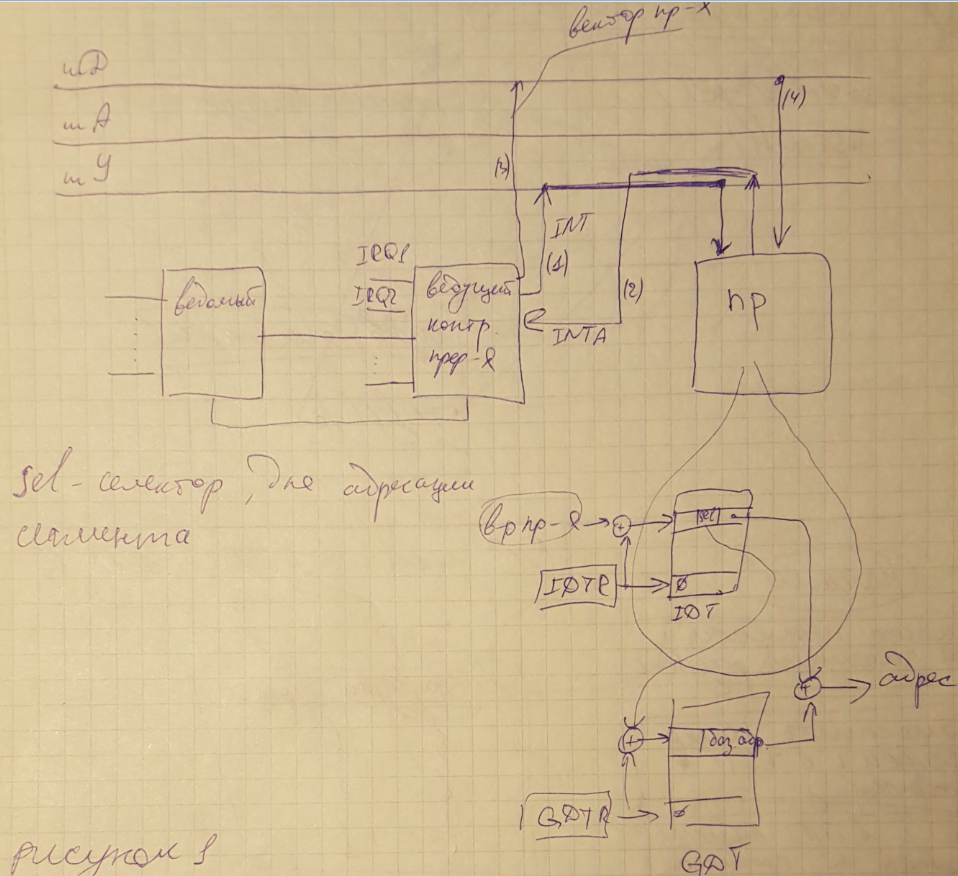
\includegraphics[width=\textwidth]{pic/3.png}
    \caption{pic}
\end{figure}

Прерывание системного таймера – единственное независимое от процессора действие в системе. В многопроцессной системе разделения времени на таймер возлагается задача декремента кванта (найти инфу про то, что частота большая, а тики всего лишь 18 раз в секунду)

Процессор проверяет наличие прерывания на своей ножке  в конце цикла выполнения каждой команды.

\begin{figure}[H]
    \centering
    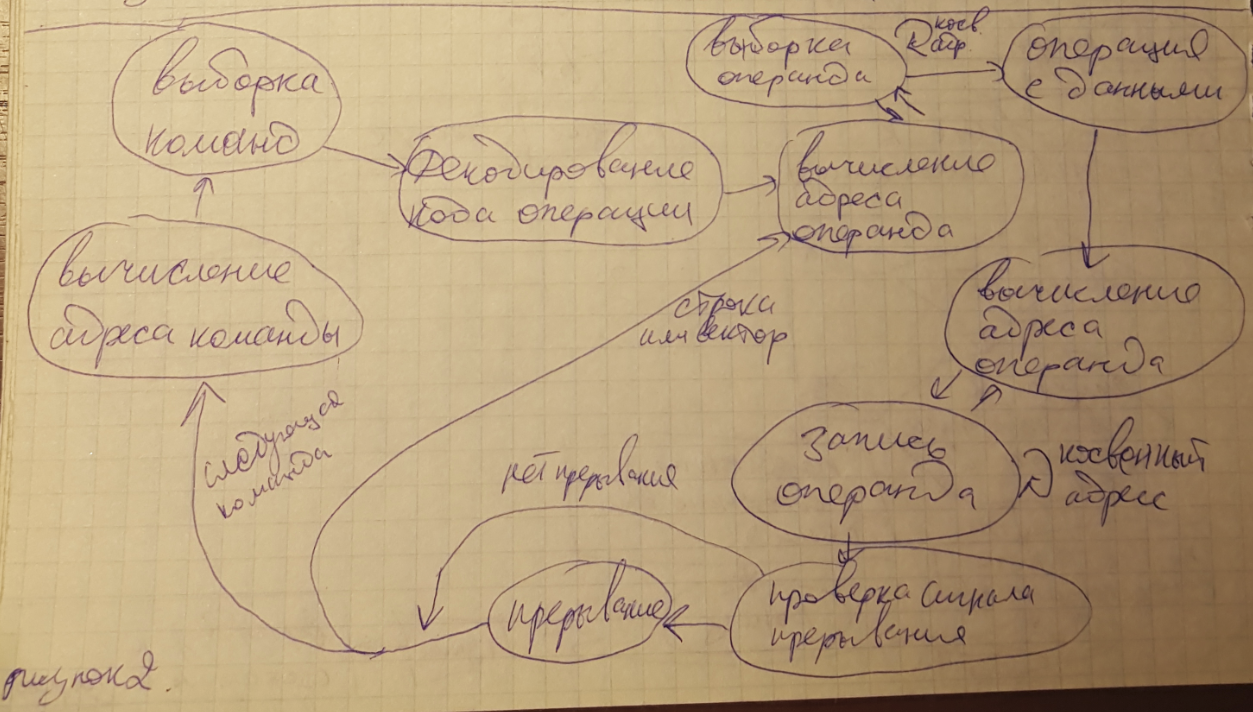
\includegraphics[width=\textwidth]{pic/4.png}
    \caption{pic}
\end{figure}

Если пришло прерывание, то сохраняется аппаратный контекст выполняемой программы. В счетчики команд устанавливается адрес обработчика прерываний. Система переключается в режим ядра.
Обработчики прерываний в системе это одна из точек входа драйвера. Это программа, которая в системе управляет работой внешнего устройства до какого то момента. Предназначен, чтобы послать и сформировать команду для устройства. Другая задача драйвера – получить от устройства данные и вернуть их процессу, который запросил эти данные. Драйверы – многовходовые программы. Один из точек входа – обработчик прерывания.
Ни одна программа не может на прямую обратиться к устройствам ввода/вывода. Сделано из соображений безопасности. Иначе любой процесс может обратиться в любое место ОС, в частности к системным таблицам.

Оси позволяют изменять функциональность без перекомпиляции ядра. 
В windows реализовано с помощью иерархии драйверов (стек драйверов). Можно написать свой драйвер, зарегистрировать в системе, и система будет обращаться к нему. В этом стеке есть разные типы драйверов. На нижнем уровне – функциональный драйвер. Пишется разработчиками устройств. Только они знают формат данных. Имеется драйвер фильтр нижнего уровня и драйвер фильтр верхнего уровня. Изменив соответствующие коды в драйверах – фильтрах, можем изменить функциональность устройства. 
Linux предоставляет возможность написания драйверов, загружаемые модули ядра.

\section{Микроядерная архитектура}

Микроядро – модуль ОС обеспечивающий взаимодействие между процессами, диспетчеризацию процессов, первичную обработку прерываний и низкоуровневое управление памятью. Микроядро реализует взаимодействие с аппаратным уровнем вычислительной системы (внешние устройства или ОЗУ). Все остальные – самостоятельные процессы, работающие, возможно, в разных адресных пространствах. ОС состоит из набора программ, эти процессы должны взаимодействовать с процессами пользователей и друг с другом. Такое взаимодействие выполняется по модели клиент – сервер. Процессы ОС предоставляют сервис пользовательским процессам, а также могу предоставлять сервис друг другу. Взаимодействие таких процессов выполняется с помощью передачи сообщений.

\begin{figure}[H]
    \centering
    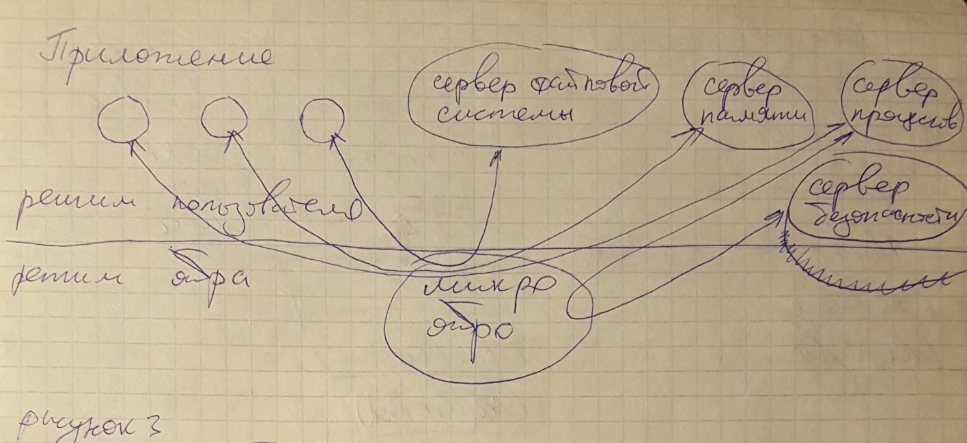
\includegraphics[width=\textwidth]{pic/5.png}
    \caption{pic}
\end{figure}

Большую часть работы, которую выполняет ОС выполняют отдельные программы, выполняющиеся в режиме пользователя.

В режиме пользователя:\\
Сервер процессов: постановка процессов в очередь, пересчет приоритетов.
Таким образом, в микроядре остаются низкоуровневые функции. 

Эффективность микроядерной архитектуры:
см. диаграмму трех состояний блокировки процесса при передаче сообщений. Там сказали, что время этих блокировок нельзя предсказать, это вероятностные вещи. Очевидно, что передача сообщений связана с неконтролируемыми задержками. А так же контролируемыми временными затратами, в частности в микроядерной архитектуре больше переключений в режим ядра (как минимум в 2 раза).

\begin{figure}[H]
    \centering
    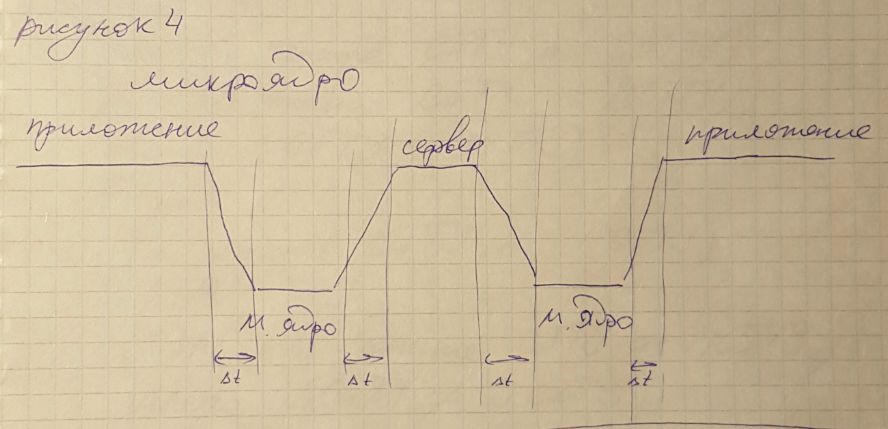
\includegraphics[width=\textwidth]{pic/6.png}
    \caption{pic}
\end{figure}

В результате микроядерная архитектура является не эффективной.